\documentclass[a4paper,12pt]{article}
\usepackage{graphicx}
\usepackage{bm,amssymb}
\usepackage{mathrsfs}
\usepackage[unicode,colorlinks=true,filecolor=blue, menucolor=black, linkcolor=black, citecolor=black,pagebackref=white]{hyperref}
\usepackage[utf8]{inputenc}
\usepackage[russian]{babel}
\usepackage{amsmath}
\usepackage{feynmp}
\usepackage{caption}
\usepackage{cite}
\usepackage[left=2cm,right=2cm, top=2cm,bottom=2cm,bindingoffset=0cm]{geometry}
\begin{document}
\title{Семинар по теме: <<Дифференциальные уравнения с малым параметром>>}
\maketitle

\subsection*{Исследование гармонического осцилятора с возбуждающей силой}

Найдём общее решение дифференциального уравнения гармонического осциллятора
с произвольной возмущающей силой:
\[
\ddot{x}+\omega^{2}x=\phi(t)
\]

 \noindent
Для этого воспользуемся методом вариации постоянных. Используя решение
однородного уравнения (с $\phi(t)\equiv0$), запишем подстановку в
виде:
\[
x(t)=C_{1}(t)\cos\omega t+C_{2}(t)\sin\omega t
\]

 \noindent
Очевидно, что поставленная так задача избыточна (имеются целых 2 произвольных
функции). Для того, чтобы задача имела однозначное решение, наложим
дополнительные ограничения. А именно, потребуем, чтобы при дальнейших
дифференцированиях члены с первыми производными констант пропадали:

\[
\dot{x}=\dot{C}_{1}\cos\omega t-\omega C_{1}\sin\omega t+\dot{C}_{2}\sin\omega t+\omega C_{2}\cos\omega t
\]

 \noindent
Поэтому требуем:

\[
\dot{C}_{1}\cos\omega t+\dot{C}_{2}\sin\omega t\equiv0\Rightarrow\dot{x}=-\omega C_{1}\sin\omega t+\omega C_{2}\cos\omega t
\]

 \noindent
Дифференцируем:

\[
\ddot{x}=-\omega\dot{C}_{1}\sin\omega t-\omega^{2}C_{1}\cos\omega t+\omega\dot{C}_{2}\cos\omega t-\omega^{2}C_{2}\sin\omega t
\]

 \noindent
Подставляем в уравнение; получаем, вместе с дополнительным условием, затребованном выше:

\[
\begin{cases}
\dot{C}_{1}\cos\omega t+\dot{C}_{2}\sin\omega t & =0\\
\dot{C}_{1}\left(-\omega\sin\omega t\right)+\dot{C}_{2}\left(\omega\cos\omega t\right) & =\phi\left(t\right)
\end{cases}
\]
\[
\begin{cases}
\dot{C}_{1} & =-\frac{1}{\omega}\phi(t)\sin\omega t\\
\dot{C}_{2} & =\frac{1}{\omega}\phi(t)\cos\omega t
\end{cases}\Rightarrow
\begin{cases}
C_{1} & =-\frac{1}{\omega}\intop_{0}^{t}\phi(\tau)\sin\omega\tau d\tau+\tilde{C}_{1}\\
C_{2} & =\frac{1}{\omega}\intop_{0}^{t}\phi(\tau)\cos\omega\tau d\tau+\tilde{C}_{2}
\end{cases}
\]

 \noindent
Значит, решение исходного неоднородного уравнения записывается как:
\[
x\left(t\right)=C_{1}\sin\omega t+C_{2}\cos\omega t+\frac{1}{\omega}\intop_{0}^{t}\sin\omega(t-\tau)\phi(\tau)d\tau
\]

 \noindent
Интересно, что такой вид ответа --- общий. Решение всякого неоднородного
линейного уравнения можно записать в виде:
\[
x(t)=x_{0}(t)+\int_{t_0}^{t}G(t,\tau)\phi(\tau)d\tau
\]

 \noindent
(где $x_{0}(t)$ --- решение однородного уравнения; а постоянную $t_0$ можно выбрать произвольной); причём если уравнение
однородно по времени (не зависит явно от времени), то $G(t,\tau)\equiv G(t-\tau)$.
Функция $G(t,\tau)$ называется функцией Грина этого уравнения.


\subsection*{Задача 1 (теория возмущений)}

При помощи изложенного выше метода можно исследовать задачи с возмущением.
Исследуем задачу:
\[
\begin{cases}
\ddot{x}+\omega^{2}x & =-\epsilon\omega^{2}x\\
x\left(0\right) & =a\\
\dot{x}\left(0\right) & =0
\end{cases}
\]



\subsubsection*{Решение}

Точное её решение записывается как:
\begin{multline*}
x(t)=a\cos(\sqrt{1+\epsilon}\omega t)\approx a\cos\left(\left(1+\frac{1}{2}\epsilon-\frac{1}{8}\epsilon^{2}\right)\omega t\right)
\approx \\
\approx a\cos\omega t-\frac{1}{2}\epsilon\omega ta\sin\omega t-\frac{1}{8}\epsilon^{2}a(\omega t\sin\omega t-\omega^{2}t^{2}\cos\omega t)
\end{multline*}

 \noindent
Эта асимптотика работет на временах $\epsilon\omega t\ll1$. На примере
этой простой задачи продемонстрируем, как разложение по $\epsilon$
можно получить по-другому, используя метод итераций. Если мы подставим
решение в виде $x(t)=x_{0}(t)+\epsilon x_{1}(t)+\epsilon^{2}x_{2}(t)+\dots$
и соберём члены с одинаковыми степенями $\epsilon$, то мы получим
систему уравнений:
\[
\ddot{x}_{k}+\omega^{2}x_{k}=-\omega^{2}x_{k-1}
\]

 \noindent
Система уравнений в таком виде позволяет построить итерационный процесс,
находя поправки высших порядков по $\epsilon$. Используя метод, изложенный
выше, можно записать:
\[
x_{k}(t)=-\omega\int_{0}^{t}\sin\omega(t-\tau)x_{k-1}(\tau)d\tau
\]

 \noindent
Начальное приближение записывается как $x_{0}(t)=a\cos\omega t$.
Таким образом, первая поправка находится как:
\[
x_{1}\left(t\right)=-\omega\int_{0}^{t}\sin\omega(t-\tau)a\cos\omega\tau d\tau=-\frac{1}{2}a\omega t\sin\omega t
\]

 \noindent
Мы видим, что эта поправка совпадает с точным разложением. Вторая
поправка:
\[
x_{2}(t)=-\omega\int_{0}^{t}\sin\omega(t-\tau)\left(-\frac{1}{2}a\omega\tau\sin\omega\tau\right)d\tau=\frac{1}{8}a\omega^{2}t^{2}\cos\omega t-\frac{1}{8}a\omega t\sin\omega t
\]

 \noindent
Исходя из этого, с точностью до $\epsilon^{2}$ мы получаем ответ
(конечно, совпадающий с разложением точного ответа, полученного выше):
\[
x(t)\approx a\cos\omega t-\epsilon\cdot\frac{1}{2}a\omega t\sin\omega t+\epsilon^{2}\cdot\frac{1}{8}a\omega t(\omega t\cos\omega t-\sin\omega t)
\]

 \noindent
Повторимся, что эта асимптотика работает на сравнительно малых временах,
при условии $\omega t\ll\epsilon^{-1}$. Способ получения асимптотик,
работающих на больших временах, включает в себя выделение ``быстрых''
и ``медленных'' степеней свободы; этот способ был изложен в лекции,
а также частично будет изложен ниже.


\subsection*{Задача 2 (ангармонический осциллятор)}

Расмотрим приближенное решение уравнения:
\[
\begin{cases}
\ddot{x}+\omega^{2}x & =-\epsilon x^{3}\\
x(0) & =a\\
\dot{x}(0) & =0
\end{cases}
\]



\subsubsection*{Решение}

Метод, изложенный в задаче 1, можно применить и тут. Раскладывая по
малости $\epsilon$ решение в виде $x(t)=x_{0}(t)+\epsilon x_{1}(t)$,
мы получаем следующую систему уравнений, дающую нам первый шаг итерационного
процесса:

\[
\begin{cases}
\ddot{x}_{0}+\omega^{2}x_{0} & =0\\
\ddot{x}_{1}+\omega^{2}x_{1} & =-x_{0}^{3}
\end{cases}
\]

 \noindent
Первое уравнение опять имеет такое же невозмущенное решение $x_{0}(t)=a\cos\omega t$;
решение второго уравнения записывается с помощью функции Грина:
\[
x_{1}\left(t\right)=-\frac{1}{\omega}\int_{0}^{t}\sin\omega(t-\tau)\cdot a^{3}\cos^{3}\omega\tau\cdot d\tau=-\frac{a^{3}}{\omega}\int_{0}^{t}[\sin\omega t\cos\omega\tau-\sin\omega\tau\cos\omega t]\cos^{3}\omega\tau\cdot d\tau
\]
Интегрируя, и используя формулы понижения степени, мы приходим к результату:
\[
x_{1}(t)=-\frac{a^{3}}{\omega^{2}}\left(\frac{3}{8}\omega t\sin\omega t+\frac{1}{32}\cos\omega t-\frac{1}{32}\cos3\omega t\right)
\]

 \noindent
Мы получили интересный физический результат: в нелинейном осциляторе
появилось колебание с третьей гармоникой (то есть с частотой $3\omega$
вместо $\omega$).


\subsection*{Задача 3 (параметрический резонанс)}

Рассмотрим теперь уравнение:

\[
\begin{cases}
\ddot{x}+\omega^{2}x & =-\epsilon x\cos\Omega t\\
x(0) & =a\\
\dot{x}(0) & =0
\end{cases}
\]

 \noindent
в условиях близости к параметрическому резонансу $\Omega=2\omega-\gamma$
($\gamma\lesssim\frac{\epsilon}{2\omega}$, $\epsilon\ll\omega^{2}$)


\subsubsection*{Решение}

Будем искать решение в виде:
\[
x(t)=A(t)\cos(\omega t+\phi(t))
\]

 \noindent
Формальная подстановка даёт:
\[
\dot{x}=\dot{A}\cos(\omega t+\phi)-A(\omega+\dot{\phi})\sin\left(\omega t+\phi\right)
\]
\[
\ddot{x}=\ddot{A}\cos(\omega t+\phi)-2\dot{A}(\omega+\dot{\phi})\sin(\omega t+\phi)-(\omega+\dot{\phi})^{2}A\cos(\omega t+\phi)-A\ddot{\phi}\sin(\omega t+\phi)
\]

 \noindent
Получаем:
\begin{multline*}
\ddot{A}\cos(\omega t+\phi)-2\dot{A}(\omega+\dot{\phi})\sin(\omega t+\phi)-\\
-\left(2\omega\dot{\phi}+\dot{\phi}^{2}\right)A\cos(\omega t+\phi)-A\ddot{\phi}\sin(\omega t+\phi)=-\epsilon A\cos(\omega t+\phi)\cos\Omega t
\end{multline*}

 \noindent
Правую часть можно представить в виде $\frac{1}{2}\left(\cos\left(\omega t+\phi+\Omega t\right)+\cos\left(\Omega t-\omega t-\phi\right)\right)$.
При $\Omega\sim2\omega$, первый член будет близок к $\cos3\omega t$.
В этом смысле он отвечает за третью гармонику и нас не интересует;
выбросим его. Получаем:
\begin{multline*}
\ddot{A}\cos(\omega t+\phi)-2\dot{A}(\omega+\dot{\phi})\sin(\omega t+\phi)-\\
-(2\omega\dot{\phi}+\dot{\phi}^{2})A\cos(\omega t+\phi)-A\ddot{\phi}\sin(\omega t+\phi)=-\frac{\epsilon A}{2}\cos(\omega t+\gamma t-\phi)
\end{multline*}

 \noindent
Из структуры уравнения видно, что если взять $\phi=\frac{\gamma t}{2}+\varphi$,
все тригонометрические функции будут одного и того же вида (осциллировать
с одинаковой частотой). Поэтому, обозначив $\omega^{\prime}=\omega+\frac{\gamma}{2}$:
\begin{multline*}
\ddot{A}\cos(\omega^{\prime}t+\varphi)-2\dot{A}(\omega^{\prime}+\dot{\varphi})\sin(\omega^{\prime}t+\varphi)-\\
-\left(2\omega\left(\frac{\gamma}{2}+\dot{\varphi}\right)+\left(\frac{\gamma}{2}+\dot{\varphi}\right)^{2}\right)A\cos(\omega^{\prime}t+\varphi)-A\ddot{\varphi}\sin(\omega^{\prime}t+\varphi)=-\frac{\epsilon A}{2}\cos(\omega^{\prime}t-\varphi)
\end{multline*}

 \noindent
Собирая члены при ``быстрых'' осциллирующих функциях $\cos\omega^{\prime}t$
и $\sin\omega^{\prime}t$, мы получаем следующую систему:

\[
\ddot{A}\cos\varphi-2\dot{A}(\omega^{\prime}+\dot{\varphi})\sin\varphi-\left(2\omega\left(\frac{\gamma}{2}+\dot{\varphi}\right)+\left(\frac{\gamma}{2}+\dot{\varphi}\right)^{2}\right)A\cos\varphi-A\ddot{\varphi}\sin\varphi =-\frac{\epsilon A}{2}\cos\varphi
\]
\[
-\ddot{A}\sin\varphi-2\dot{A}(\omega^{\prime}+\dot{\varphi})\cos\varphi+\left(2\omega\left(\frac{\gamma}{2}+\dot{\varphi}\right)+\left(\frac{\gamma}{2}+\dot{\varphi}\right)^{2}\right)A\sin\varphi-A\ddot{\varphi}\cos\varphi =-\frac{\epsilon A}{2}\sin\varphi
\]

 \noindent
Мы ожидаем, что $A$ и $\varphi$ - медленные переменные; это означает,
что всякое дифференцирование этих переменных должно давать дополнительную
малость. В ведущем прибижении это позволяет выбросить члены $\ddot{A}$,
$\ddot{\varphi}$, $\dot{\varphi}^{2}$ и $\dot{A}\cdot\dot{\varphi}$
(те, в которых производных две). Кроме того, имеется просто малость
$\gamma\ll\omega$. Это позволяет нам сильно упростить систему:

\[
\begin{cases}
-2\dot{A}\omega^{\prime}\sin\varphi-\omega(\gamma+2\dot{\varphi})A\cos\varphi & =-\frac{\epsilon A}{2}\cos\varphi\\
-2\dot{A}\omega^{\prime}\cos\varphi+\omega(\gamma+2\dot{\varphi})A\sin\varphi & =-\frac{\epsilon A}{2}\sin\varphi
\end{cases}
\]

 \noindent
Заметим, что решение $\varphi={\rm const}$ удовлетворяет этому уравнению,
если $\tan^{2}\varphi=\frac{\epsilon-2\omega\gamma}{\epsilon+2\omega\gamma}$.
При этом оставшееся уравнение на $A$ записывается как:

\[
\dot{A}=A\frac{\sqrt{\epsilon^{2}-(2\omega\gamma)^{2}}}{4\omega}\Rightarrow A(t)\simeq C\exp\left(\frac{1}{4}\sqrt{\frac{\epsilon^{2}-(2\omega\gamma)^{2}}{\omega^{2}}}t\right)
\]

 \noindent
Во-первых видно, что резонанс пропадает при достаточно сильном несовпадении
частот $\Omega$ и $2\omega$ (а именно, условие записывается как
$\gamma<\frac{\epsilon}{2\omega}$). При большем отклонении частоты
мы не получим резонанс (то есть экспоненциальный рост), а получим
биения ограниченной амплитуды. \\\\
Чтобы получить этот ответ, мы сделали предположения, а именно - мы
предполагали ``медленность'' функций $A(t)$ и $\varphi(t)$; из
этих предположений мы получили приближенное решение, которое эти предположения
подтверждает. Таким образом, наше приближенное решение нашей системы
непротиворечиво.

\begin{figure}[h]
\caption{Численное решение уравнения с параметрическим резонансом при условиях
$\omega=10$, $\epsilon=1$, $\gamma=0$; жёлтая линия - экспоненциальная
огибающая $\sim\exp\left(\frac{\epsilon t}{4\omega}\right)$}
\centering
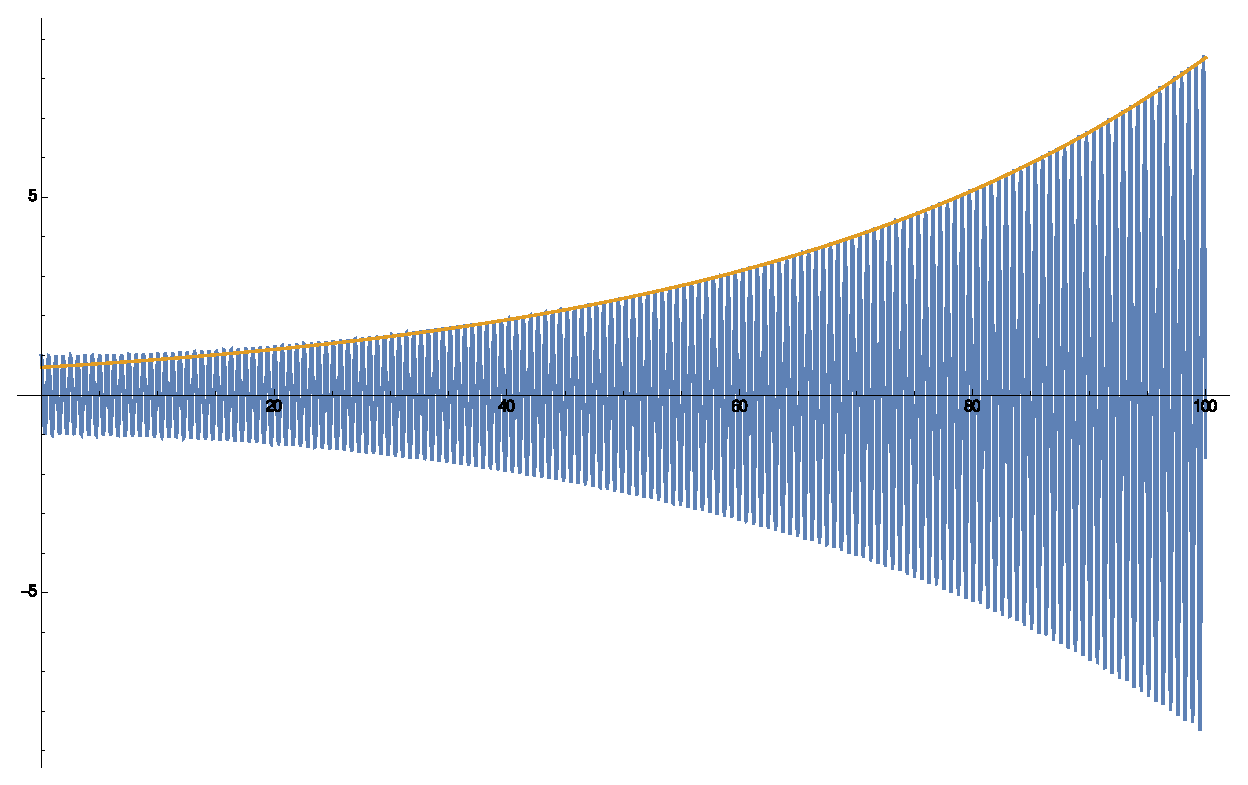
\includegraphics[width=0.5\columnwidth]{paramresonance.eps}
\end{figure}


\subsection*{Задачи для домашнего решения}

\noindent \textbf{Упражнение 1}

\noindent Частица с зарядом $q>0$ налетает на неподвижную частицу с зарядом $Q>0$ с прицельным параметром $b$. Оцените угол отклонения частицы от исходного направления, считая частицу очень быстрой $mv^{2}/2\gg qQ/b$.

\vspace{15pt}
\noindent \textbf{Упражнение 2}

\noindent Рассмотрите уравнение
\begin{equation}\notag
\ddot{x}+\kappa\dot{x}^{2}+\omega^{2}x	=0
\end{equation}
\noindent с начальным условием: $x(0)=a,\quad\dot{x}(0)=0$ при $\kappa a\ll 1$.
\noindent Найдите главную поправку к невозмущенному решению ($\kappa=0$), работающую при малых временах. При каком $t$ такое приближенное решение перестает работать?

\vspace{15pt}
\noindent \textbf{Упражнение 3}

\noindent Рассмотрите уравнение
\begin{equation}\notag
\ddot{x}+\omega^{2}x	=\epsilon x^{4}
\end{equation}
\noindent c начальным условием $x(0)=0$,$\quad\dot{x}(0)=\omega a$ при $\epsilon a^{3}\ll\omega^{2}$.
\noindent Найдите главную поправку к невозмущенному решению ($\epsilon=0$), работающую при малых временах. При каком $t$ такое приближенное решение перестает работать?

\vspace{15pt}
\noindent \textbf{Упражнение 4}

\noindent Найдите функцию Грина уравнения
\begin{equation}\notag
\ddot{x}+\gamma\dot{x}	=\phi(t).
\end{equation}

\noindent Для этого рассмотрите задачу
\begin{equation}\notag
\phi(t)	\rightarrow0,\quad t\rightarrow-\infty,
\end{equation}
\begin{equation}\notag
x(-\infty)	=0,\quad\dot{x}(-\infty)=0
\end{equation}
и решитие ее методом вариации постоянной.

\vspace{15pt}
\noindent \textbf{Задача 1}

\noindent Используя найденную функцию Грина найдите приближенно решение уравнения из упражнения 3 для
\begin{equation}\notag
\phi(t)	=\phi_{0}\frac{\tau}{\tau^{2}+t^{2}},
\end{equation}
\begin{equation}\notag
x(-\infty)	=0,\quad\dot{x}(-\infty)=0
\end{equation}
\noindent при $\tau\ll\gamma^{-1}\ll t$.

\noindent В таком случае решение можно представить в виде
\begin{equation}\notag
x(t)	=C\left(1+a_{1}\frac{\tau}{t}+a_{2}\frac{\tau}{t}\frac{1}{\gamma t}+...\right)
\end{equation}

\noindent Определите $C$, $a_{1}$, $a_{2}$.\\\\

\vspace{15pt}
\noindent \textbf{Задача 2}

\noindent Частица массы $m$ движется в потенциале $U(x)=-U_{0}\cos\left(x/a\right)$. Помимо этого на частицу действуют сила вязкого трения -$\gamma m\dot{x}$ и постоянная сила $F$. Пока сила $F>U_{0}/a$, у частицы имеется режим движения с постоянной средней скоростью. Если силу постепенно уменьшать, то из-за инерции этот режим может сохраниться вплоть до некоторого критического значения $F_{c}$. Найдите значение $F_{c}$ в случае малого трения и определите критерий применимости ответа.
\end{document}
